% ------------------------------ Related Studies -----------------------------

\section{Related Studies}

\begin{comment}
    For avoiding plagiarism, citations should be used for all referred texts particularly here and other parts of the document using appropriate numbers within square bracket for all mapped references under \textbf{References} section. You should check any standard journal paper for typical use of citations.     
\end{comment}

\vspace{-2em}

\begin{table}[H]
    \centering
    \label{tab:related_studies}
    \setlength{\arrayrulewidth}{1pt}
    \arrayrulecolor{black}
    \begin{tabularx}{\textwidth}{|p{3.5cm}|X|}
    \hlineB{1.0}
    \rowcolor{lightestgray}
    \textbf{Study} & \textbf{Summary} \\ \hlineB{1.0}
    Choudhury et al. (2013) & Explored the predictive capabilities of social media content in identifying depression by analyzing Twitter data. They discovered that specific linguistic patterns (e.g., negative emotion words) correlated strongly with self-reported depressive symptoms \cite{Choudhury2013PredictingDV}. \\ \hlineB{1.0}
    Guntuku et al. (2017) & Conducted an integrative review which synthesized various methodologies highlighted that social media platforms are rich sources of data, revealing critical information about users' mental health \cite{Guntuku2017DetectingDA}. \\ \hlineB{1.0}
    Mathur et al. (2022) & Provided a systematic review analysing machine learning techniques for mental health detection using social media data, leveraging both individual assessments and broader epidemiological studies \cite{Mathur2022MentalHC}. \\ \hlineB{1.0}
    Nadeem (2016) & Investigated depression identification on Twitter by developing algorithms to discern emotional cues in tweets revealing that simple text analysis could lead to improvements in identifying mental risks \cite{nadeem2016identifying}. \\ \hlineB{1.0}
    AlSagri and Ykhlef (2020) & Introduced a machine learning–based approach for depression detection on Twitter that combined both content and activity features. Their work demonstrated that a fusion of linguistic and behavioral analysis can enhance the accuracy of depression identification \cite{alsagri2020machine}. \\ \hlineB{1.0}
    Vaishnavi et al. (2022) & Examined various machine learning algorithms for predicting mental health illnesses using social media posts. Their findings emphasized that certain algorithms outperform others in classifying mental health conditions, underlining the importance of algorithm selection \cite{Vaishnavi_2022}. \\ \hlineB{1.0}
    Safa et al. (2023) & Presented a roadmap for predicting mental health using social media, highlighting ongoing challenges such as ethical considerations and data privacy. They stressed the need for a robust ethical framework in research that leverages social media data \cite{safa2023predictingmentalhealthusing}. \\ \hlineB{1.0}
    Ensemble learning using transformers for NLP & Provided a comprehensive review of transformer models (BERT, XLNet, RoBERTa, GPT-2, ALBERT) across multiple NLP tasks. The study introduced ensemble learning with these models and demonstrated that ensemble approaches can significantly improve performance over single classifier methods \cite{Zhang_2024}. \\ \hlineB{1.0}
    Ensemble hybrid model for depression detection & Proposed an ensemble hybrid model combining SVM and MLP to improve depression prediction accuracy. Addressing class imbalance with SMOTE and cluster sampling, the model achieved an accuracy of 99.39\% and an F1-score of 99.51\%, outperforming previous approaches \cite{Saha2024}. \\ \hlineB{1.0}
    Single classifier vs. ensemble ML \newline approaches & Explored various ML techniques to predict mental health issues using survey responses from OSMI. The study compared single classifiers with ensemble approaches, finding that Gradient Boosting achieved the highest accuracy \cite{Chung_2023}. 
    \\ \hlineB{1.0}
\end{tabularx}
\end{table}


% ----- add pre frame study

\begin{comment}
    
\begin{figure}[H]  
    \centering
    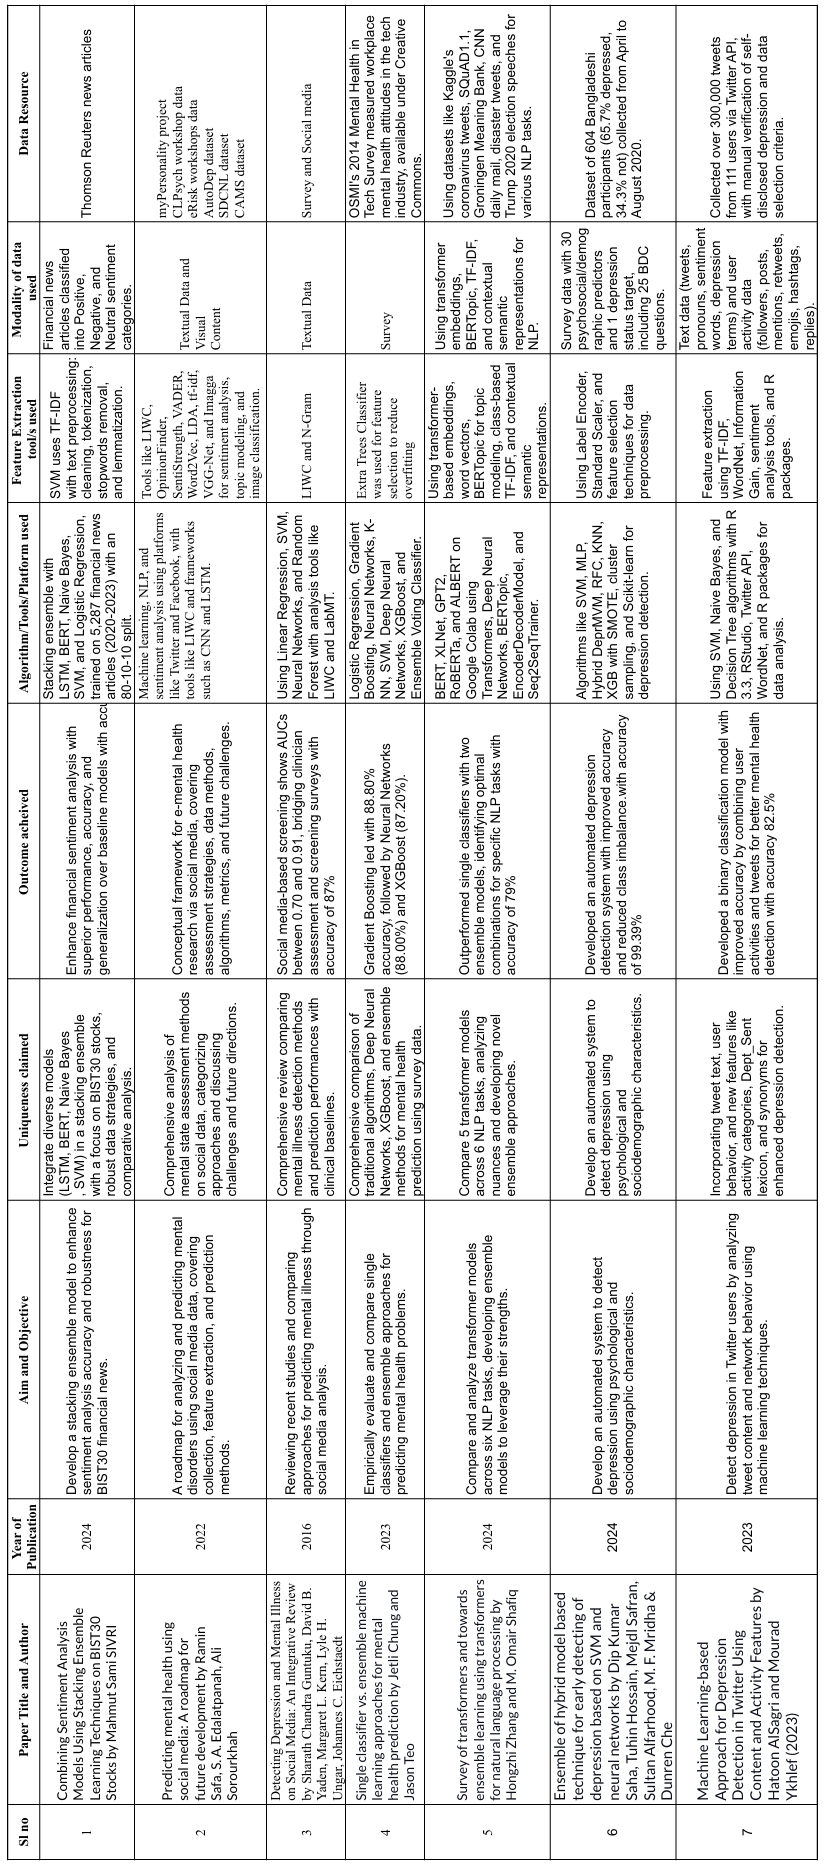
\includegraphics[width=0.95\textwidth]{Images/preframe-study.png}  
    \caption*{Pre frame study review}
    \label{Preframe Study Review}  % Label for referencing the figure
\end{figure}

\end{comment}




\pagebreak

\vspace*{-3.0em}

% Force the rotated table right here
\begin{figure}[H]
\centering

%\caption*{\scriptsize Preframe Study Review}
\hspace*{-0.4cm}
\rotatebox{90}{
\begin{minipage}{\textheight} % Use textheight as width due to rotation
\tiny  % Or \scriptsize or even smaller
\setlength{\arrayrulewidth}{1pt} % Bold vertical lines
\begin{tabular}{|>{\raggedright\arraybackslash}m{0.6cm}|>{\raggedright\arraybackslash}m{2.5cm}|>{\raggedright\arraybackslash}m{0.6cm}|>{\raggedright\arraybackslash}m{2.4cm}|>{\raggedright\arraybackslash}m{2.4cm}|>{\raggedright\arraybackslash}m{2.4cm}|>{\raggedright\arraybackslash}m{2.2cm}|>{\raggedright\arraybackslash}m{2.4cm}|>{\raggedright\arraybackslash}m{2.2cm}|>{\raggedright\arraybackslash}m{2.2cm}|>{\raggedright\arraybackslash}m{2.4cm}|}
%\hlineB{1.0}
%\hlineB{1.4}
\multicolumn{10}{c}{\footnotesize \textbf{PREFRAME STUDY REVIEW}} \\
\hlineB{1.4}
\rowcolor{lightestgray}
\textbf{\rule{0pt}{1.5em} SI No.} & \textbf{\rule{0pt}{1.5em} Paper Title and Author} & \textbf{\rule{0pt}{1.5em} Year} & \textbf{\rule{0pt}{1.5em} Aim and Objective} & \textbf{\rule{0pt}{1.5em} Uniqueness Claimed} & \textbf{\rule{0pt}{1.5em} Outcome Achieved} & \textbf{\rule{0pt}{1.5em} Algorithm/Tools} & \textbf{\rule{0pt}{1.5em} Feature Extraction} & \textbf{\rule{0pt}{1.5em} Modality of Data} & \textbf{\rule{0pt}{1.5em} Data Resource} \\ 
\hlineB{1.4}
1 & Combining Sentiment Analysis Models Using Stacking Ensemble Learning Techniques on BIST30 Stocks by Mahmut Sami SIVRI & 2024 & Develop a stacking ensemble model to enhance sentiment analysis accuracy and robustness for BIST30 financial news. & Integrate diverse models (LSTM, BERT, Naive Bayes, SVM) in a stacking ensemble with a focus on BIST30 stocks, robust data strategies, and comparative analysis. & Enhance financial sentiment analysis with superior performance, generalization over baseline models with accuracy of 85\% & Stacking ensemble with LSTM, BERT, Naive Bayes, SVM, and Logistic Regression, trained on 5,287 financial news articles (2020-2023) with an 80-10-10 split. & SVM uses TF-IDF with text preprocessing: cleaning, tokenization, stopwords removal, and lemmatization. & Financial news articles classified into Positive, Negative, and Neutral sentiment categories. & Thomson Reuters news articles \\ 
\hlineB{1.4}

2 & Predicting mental health using social media: A roadmap for future development by Ramin Safa, S. A. Edalatpanah, Ali Sorourkhah & 2022 & A roadmap for analyzing and predicting mental disorders using social media data, covering collection, feature extraction, and prediction methods. & Comprehensive analysis of mental state assessment methods on social data, categorizing approaches and discussing challenges and future directions. & Conceptual framework for e-mental health research via social media, covering assessment strategies, data methods, algorithms, metrics, and future challenges. & Machine learning, NLP, and sentiment analysis using platforms like Twitter and Facebook, with tools like LIWC and frameworks such as CNN and LSTM. & Tools like LIWC, OpinionFinder, SentiStrength, VADER, Word2Vec, LDA, tf-idf, VGG-Net, and Imagga & Textual Data and Visual Content & myPersonality project CLPsych workshop data, eRisk workshops data, AutoDep dataset, SDCNL dataset, CAMS dataset  \\
\hlineB{1.4}

3 & Detecting Depression and Mental Illness on Social Media: An Integrative Review by Sharath Chandra Guntuku, David B. Yaden, Margaret L. Kern, Lyle H. Ungar, Johannes C. Eichstaedt & 2016 & Reviewing recent studies and comparing approaches for predicting mental illness through social media analysis. & Comprehensive review comparing mental illness detection methods and prediction performances with clinical baselines. & Social media-based screening shows AUCs between 0.70 and 0.91, bridging clinician assessment and screening surveys with accuracy of 87\% & Using Linear Regression, SVM, Neural Networks, and Random Forest with analysis tools like LIWC and LabMT. & LIWC and N-Gram & Textual Data  & Survey and Social media \\
\hlineB{1.4}

4 & Single classifier vs. ensemble machine learning approaches for mental health prediction by Jetli Chung and Jason Teo & 2023 & Empirically evaluate and compare single classifiers and ensemble approaches for predicting mental health problems. & Comprehensive comparison of traditional algorithms, Deep Neural Networks, XGBoost, and ensemble methods for mental health prediction using survey data. & Gradient Boosting led with 88.80\% accuracy, followed by Neural Networks (88.00\%) and XGBoost (87.20\%). & Logistic Regression, Gradient Boosting, Neural Networks, K-NN, SVM, Deep Neural Networks, XGBoost, and Ensemble Voting Classifier. & Extra Trees Classifier was used for feature selection to reduce overfitting & Survey & OSMI's 2014 Mental Health in Tech Survey measured workplace mental health attitudes in the tech industry, available under Creative Commons. \\
\hlineB{1.4}

5 & Survey of transformers and towards ensemble learning using transformers for natural language processing by Hongzhi Zhang and M. Omair Shafiq & 2024 & Compare and analyze transformer models across six NLP tasks, developing ensemble models to leverage their strengths. & Compare 5 transformer models across 6 NLP tasks, analyzing nuances and developing novel ensemble approaches. & Outperformed single classifiers with two ensemble models, identifying optimal combinations for specific NLP tasks with accuracy of 79\% & BERT, XLNet, GPT2, RoBERTa, and ALBERT on Google Colab using Transformers, Deep Neural Networks, BERTopic, EncoderDecoderModel, and Seq2SeqTrainer. & Using transformer-based embeddings, word vectors, BERTopic for topic modeling, class-based TF-IDF, and contextual semantic representations. & Using transformer embeddings, BERTopic, TF-IDF, and contextual semantic representations for NLP. & Using datasets like Kaggle's coronavirus tweets, SQuAD1.1, Groningen Meaning Bank, CNN daily mail, disaster tweets, and Trump 2020 election speeches for various NLP tasks. \\
\hlineB{1.4}

6 & Ensemble of hybrid model based technique for early detecting of depression based on SVM and neural networks by Dip Kumar Saha, Tuhin Hossain, Mejdl Safran, Sultan Alfarhood, M. F. Mridha \& Dunren Che & 2024 & Develop an automated system to detect depression using psychological and sociodemographic characteristics. & Develop an automated system to detect depression using psychological and sociodemographic characteristics. & Developed an automated depression detection system with improved accuracy and reduced class imbalance.with accuracy of 99.39\% & Algorithms like SVM, MLP, Hybrid DeprMVM, RFC, KNN, XGB with SMOTE, cluster sampling, and Scikit-learn for depression detection. & Using Label Encoder, Standard Scaler, and feature selection techniques for data preprocessing. & Survey data with 30 psychosocial/demographic predictors and 1 depression status target, including 25 BDC questions. & Dataset of 604 Bangladeshi participants (65.7\% depressed, 34.3\% not) collected from April to August 2020. \\
\hlineB{1.4}

7 & Machine Learning-based Approach for Depression Detection in Twitter Using Content and Activity Features by Hatoon AlSagri and Mourad Ykhlef & 2023 & Detect depression in Twitter users by analyzing tweet content and network behavior using machine learning techniques. & Incorporating tweet text, user behavior, and new features like activity categories, Dept\_Sent lexicon, and synonyms for enhanced depression detection. & Developed a binary classification model with improved accuracy by combining user activities and tweets for better mental health detection with accuracy 82.5\%. & Using SVM, Naive Bayes, and Decision Tree algorithms with R 3.3, RStudio, Twitter API, WordNet, and R packages for data analysis. & Feature extraction using TF-IDF, WordNet, Information Gain, sentiment analysis tools, and R packages. & Text data (tweets, pronouns, sentiment words, depression terms) and user activity data (followers, posts, mentions, retweets, emojis, hashtags, replies). & Collected over 300,000 tweets from 111 users via Twitter API, with manual verification of self-disclosed depression and data selection criteria. \\
\hlineB{1.4}

8 & Predicting Depression via Social Media" Authors : Munmun De Choudhury, Michael Gamon, Scott Counts, Eric Horvitz & 2013 & Leveraging social media behavioral patterns to detect and predict Major Depressive Disorder (MDD) early. & Pioneering crowdsourced clinical data and multifaceted behavioral analysis for early depression prediction. & Achieved 70\% accurate depression prediction, highlighting key behavioral and linguistic markers. & Utilized SVM with RBF kernel, PCA, and 10-fold cross-validation on Twitter data for depression analysis. & Employed LIWC, ANEW, and custom lexicons for linguistic, emotional, and medication-related feature extraction. & Analyzed Twitter posts, surveys (CES-D, BDI), demographics, and social network data for depression detection. & Collected data from 1,583 U.S.-based crowdworkers, analyzed 2M+ tweets and surveys (CES-D, BDI) with strict quality controls. \\
\hlineB{1.4}


9 & Predicting Mental Health Illness using Machine Learning Algorithms by Konda Vaishnavi & 2022 & Evaluate and compare machine learning techniques for accurate mental health issue prediction. & Unique comparison of five ML techniques for mental health prediction using diverse accuracy metrics and ROC curves. & Achieved 81.75\% accuracy with stacking, with all classifiers showing strong ROC values (0.8–0.9). & Utilized Logistic Regression, K-NN, Decision Tree, Random Forest, and Stacking for mental health prediction. & Performed feature selection to reduce 27 attributes to 8 for mental health prediction. & Used a dataset with 27 attributes and 1259 entries, including text documents for mental health prediction. & Not mentioned \\
\hlineB{1.4}

10 & Generalizability of Machine Learning to Categorize Various Mental Illness Using Social Media Activity Patterns by Ang, C.S. \& Venkatachala, R. & 2023 & Explore linguistic patterns and cross-platform machine learning models for classifying mental health groups based on social media activity. & Improved accuracy by 2.11\% with simpler cross-platform models for mental health classification on Twitter and Reddit. & Achieved 91.5\% accuracy, with better Reddit model generalization and distinct linguistic patterns between platforms. & Used CNN, Word2Vec, NLTK, and Google Colab for Twitter and Reddit-based mental health classification. & Employed LIWC, Porter Stemmer, and NLTK for feature extraction in mental health classification. & Analyzed 606K Reddit posts and 23M tweets covering 6 mental health conditions from relevant subreddits and hashtags. & Used 23M Twitter tweets and 606K Reddit posts from mental health-related subreddits for cross-platform model training and testing. \\
\hlineB{1.4}

% Add more rows as needed
\end{tabular}
\end{minipage}
}
%\vspace{0.1em}
%\caption*{Preframe Study Review}
\end{figure}

% ----------------------------- Related Studies End --------------------------

\pagebreak

% ------------------------------ Related Studies -----------------------------

